\chapter{\LaTeX\ Básico}

\section{\LaTeX\ Muito Básico}

\subsection{Documento Mínimo}

Um documento mínimo \LaTeX\ tem a aparência da listagem \ref{code:latex:min}. Sua aparência é a da figura
\ref{fig:pdf:min}




\lstinputlisting[
caption={Um documento mínimo em \LaTeX.},    
label=code:latex:min,
]{minimo.tex}


\begin{figure}
        \centering
        
\includegraphics[clip,trim= 4.8cm 24.5cm 14cm 4.3cm ]{minimo.pdf}
\caption{Texto que será impresso em uma págica após o processamento do arquivo da listage \ref{code:latex:min}}
\label{fig:pdf:min}

\end{figure}

Cada documento \LaTeX\ começa com a declaração de que classe ele usa. A classe de um documento é sua principal guia de formatação/composição, sendo completada por
pacotes, que não foram usados no exemplo mínimo. Cada classe pode possuir opções, como a opção \verb|a4paper| usada no exemplo, e que define o tamanho do papel.

O símbolo de porcentagem indica o início de um comentário. Um arquivo \LaTeX tem duas áreas principais, o preâmbulo, onde são colocados os comandos de configuração da saída, e o documento propriamente dito, onde é colocado o texto.

O formato básico de um comando \LaTeX\ é:
\begin{verbatim}
\comando[<opções]{<parâmetro>}
\end{verbatim}
porém existem comandos com colchetes após os parâmetros ou mais de um parâmetro, como veremos mais adiante.

Neste texto vamos usar a classe \texttt{article}, porém é muito comum que as pessoas usem outras classes, como classes fornecidas pela editora que vai
publicar seu artigo ou livro. Classes bastante usadas são:
\begin{itemize}
    \item article, genérica para artigos
    \item report, genérica para relatórios técnicos
    \item book, genérica para livro
    \item IEEEtran, classe para publicações diversas da IEEE
\end{itemize}

Uma das facilidades fornecidas por \LaTeX\ é escrever seu artigo em uma classe genérica e depois simplesmente trocar a classe para a da editora desejada.

 Existe uma classe para os documentos acadêmicos da Coppe, mantida por um grupo de voluntários que inclui este autor, e que cobre dissertação, tese, exame de qualificação e outras coisas. Ela pode ser obtida no GitHub no endereço
 \url{https://github.com/COPPE-UFRJ/CoppeTeX/tree/master/dist}

\section{Estrutura de um documento}

Um documento \LaTeX\ utiliza uma estrutura de partes hieráquicas, que, nos principais estilos são:
    \begin{itemize}
    \item \lstinline|\part{<título>}| -- só para report e book
    \item \lstinline|\chapter{<título>}| -- só para report e book
    \item \lstinline|\section{<título>}|
    \item \lstinline|\subsection{<título>}|
    \item \lstinline|\subsubsection{<título>}|
    \item \lstinline|\paragraph{<texto>}|
    \item \lstinline|\subparagraph{<texto>}|
\end{itemize}

A listagem \ref{code:primeiro} mostra um documento usando a classe \lstinline|article| e divido em seções e subseções.
Parágrafos não marcados são separados por uma linha vazia.
Uma prática comum em \LaTeX\ é preencher um frase, da letra maiúscula ao ponto final, por linha de texto, e, obviamente, manter as linhas de um parágrafo juntas.

Apesar dos exemplos estarem gerando páginas de PDF,  como mostrado na figura \ref{fig:primeiroartigo} a maior parte
das figuras será cortada para evitar excesso de espaço em branco
neste documento.

\lstinputlisting[
caption={Um artigo básico em \LaTeX.},
label=code:primeiro,
]{primeiroartigo.tex}

\begin{figure}
    \centering
    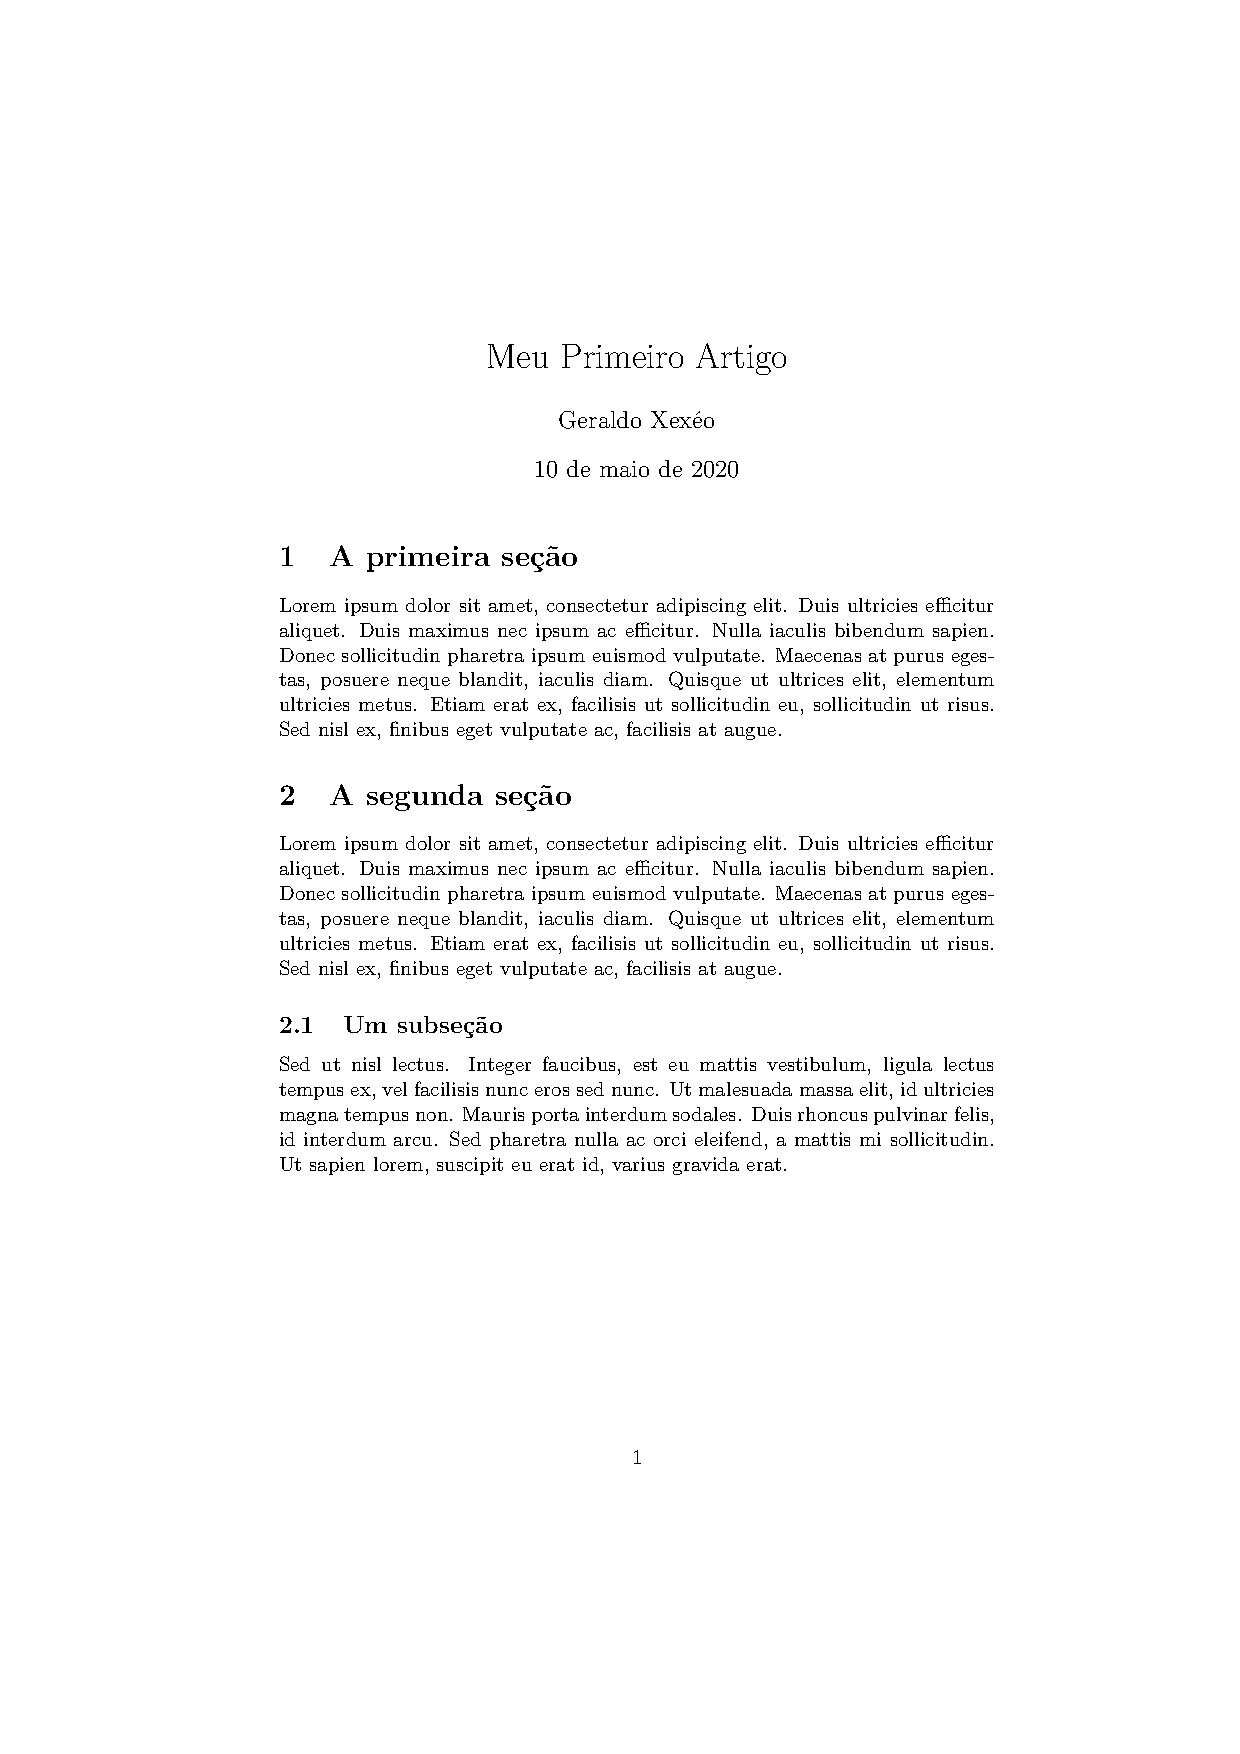
\includegraphics[height=.8\textheight,frame]{primeiroartigo}
    \caption{PDF produzido pelo texto da figura \ref{fig:latex:1a}.}
    \label{fig:primeiroartigo}
\end{figure}


\section{Informação de Capa}

Algumas informações que devem existir em um documento, que chamaremos de informação de capa ou de título, são colocadas no preâmbulo e inseridas automaticamente no documento por meio de comandos como 
\lstinline|\maketitle| ou \lstinline|\titlepage|.

Um artigo pode possuir um título, um subtítulo, um ou mais autores e uma data. A data, se não for colocada, é gerada automaticamente. A listagem \ref{code:primeiro} mostra os comandos \lstinline|title|, \lstinline|author|. O efeito deles acontece quando o comando \lstinline|maketitle| é chamado. O resultado é mostrado na figura \ref{fig:primeiroartigo}.

\section{Comandos mais comuns}

A figura \ref{fig:com:comum} mostra alguns comandos mais comuns para
formatar caracteres e seus resultados. Atenção ao uso das
linhas vazias para manter ou trocar de parágrafo:

\begin{figure}[hbt]
    \begin{LTXexample}[pos=b]
\textbf{negrito} 
\textit{itálico}

\underline{sublinhado}

\Large
Texto Grande
\normalsize

e\textsuperscript{superescrito}
e\textsubscript{subescrito}
    \end{LTXexample}
    \caption{Comandos comuns em \LaTeX}
    \label{fig:com:comum}
\end{figure}

\subsection{Fazendo referência a outra parte}

Muitas vezes em um documento é necessário citar alguma outra parte do mesmo, como uma figura, tabela ou seção. Para isso são usados dois comandos \lstinline|\label{<rótulo>}|, que cria um rótulo indicando para o local com o conhecimento do número a ser usado, como o número da figura, e \lstinline|\ref{<rótulo}|. Existe opções de citação específica como \lstinline|\pageref{<rótulo>}|, que cita a página e não o contexto.

\lstinputlisting[
caption={Artigo usando as referências.},
label=code:labelref,
]{labelref.tex}

\begin{figure}
    \centering
    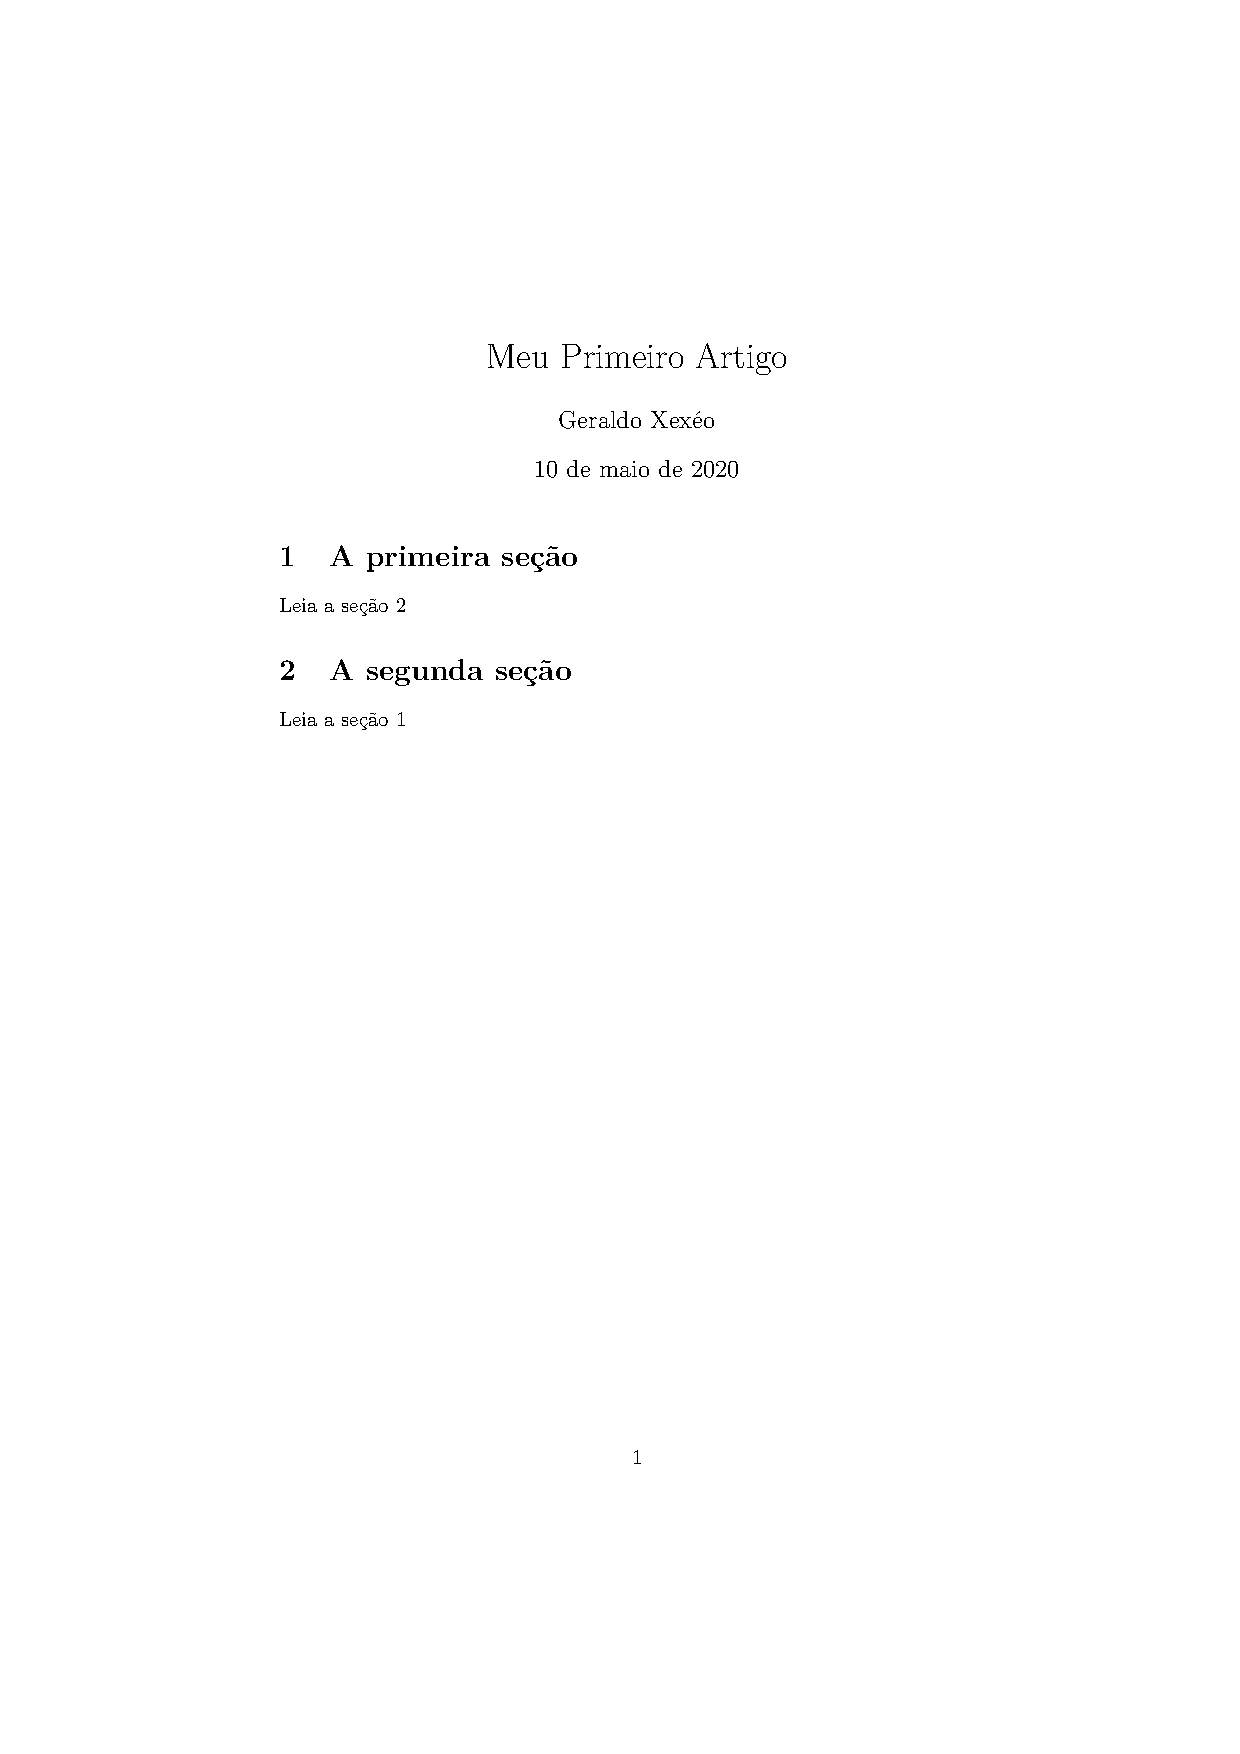
\includegraphics[height=.8\textheight,frame]{labelref}
    \caption{PDF do exemplo do uso de referências (listagem \ref{code:labelref}).}
    \label{fig:labelref}
\end{figure}


\section{Usando pacotes}

\subsection{O Que São Pacotes}
    \begin{outline}
        \1 São extensões que adicionam poder ao \LaTeX
        \1 Algumas são muito usadas
        \2 Babel -- para escrever em outras línguas
        \3 Sim, \LaTeX\ é muito focado em inglês, mas há muitos pacotes criados em outras línguas, como alemão.
        \3 Um bom pacote é auto-configurável na maioria das línguas por meio do Babel
        \3 Um ótimo pacote deixa você configurar como você quiser a língua
        \1 Comando 
        \2 \lstinline|\usepackage[<opções>]{package}|
        \1 Os bons pacotes tem várias formas de configurações nessas opções
        \1 Os bons pacotes estão vivos, isto é, são mantidos por seus autores ou seguidores
    \end{outline}

Três pacotes essenciais para escrever em português do Brasil são:
\begin{itemize}
    \item Babel
    \item inputencode
    \item fontencode
\end{itemize}


\subsection{Babel}
    \begin{outline}
    \1 Pacote que permite usar o \LaTeX\ com outras linguagens
    \1 Chamado por pacotes que escrevem algo, como a palavra ``Capítulo''
    \1 Comando 
    \2 \lstinline|\usepackage[english,brazilian]{babel}|
    \2 A última linguagem é a mais importante
    \1 A opção ``portuguese'' usa termos de Portugal, como dizer que um documento Web foi \textit{acedido} em vez de \textit{acessado}.
    \1 Usar sempre \textbf{brazilian}
\end{outline}

\subsection{inputencode}
    \begin{outline}
        \1 \lstinline|\usepackage[utf8]{inputencode}|
        \1 Faz o \LaTeX\ entender código UTF-8 nos documentos que ele lê
        \2 Caracteres acentuados do Português e outras línguas!
        \3 áéíóúâêîôûäëïöüàèìòù
        \1 Você não precisa mais usar \textbackslash´e
        \1 \textbf{Não use o utf8x}, ele morreu e tem defeitos
        \1 Melhor ainda, use o \hologo{LuaLaTeX} e dispense esse pacote!
    \end{outline}

\subsection{fontencode}
    \begin{outline}
        \1 \lstinline|\usepackage[T1]{fontencode}|
        \1 Quando gera o PDF, o \LaTeX\ por \textit{default} use o \textit{font encoding} OT1, que só tem 7 bits.
        \2 Isso faz que uma leitura do texto do PDF para indexação, por exemplo, recupere combinações de caracteres que foram geradas para representar um caracter
        \3 Isso gera problemas na indexação do seu documento, ruim para você
        \1 Garante também que as ligaduras, grande parte da beleza do texto do \TeX\ sejam geradas, pois elas não são construídas, mas sim pertencentes as fontes.
        \1 Sempre necessário
    \end{outline}

\section{Ambientes}
\subsection{O Que São Ambientes}

    \begin{itemize}
        \item Ambientes são escopos fechados que são usados para mudar, temporariamente, o comportamento do \LaTeX\
        \item Basicamente, um contexto
        \item tem início (\textbackslash begin\{nome\}) e fim (\textbackslash end\{nome\})
        \item Em geral, um comando dado dentro do ambiente deixa de ser válido fora do ambiente
        \item Tem que ser construídos um dentro do outro. São estruturados
    \end{itemize}

\subsection{Ambiente Mais Usados}
\begin{outline}
    \1 \lstinline|itemize| -- ver listagem \ref{code:labelref}
    \1 \lstinline|enumerate| -- ver listagem \ref{code:labelref}
    \1 \lstinline|equation|
    \1 \lstinline|tabular|  -- usado normalmente dentro de um ambiente table
    \1 \lstinline|abstract|
    \1 Floats -- alguns ambiente ``flutuam'' no documento,
    sendo posicionados pelo algoritmo do \LaTeX.
    \2 \lstinline|figure|
    \2 \lstinline|table|
    \2 \lstinline|lstlisting| -- depende do pacote \lstinline|listings|
\end{outline}

\subsection{Equações}

Você pode fazer equações dentro do texto, o que é conhecido no \LaTeX\ como \textit{inline}, ou em ambientes próprios, quando elas ficam isoladas, como mostrado na figura \ref{fig:eq}

\begin{figure}[hbt]
    \begin{LTXexample}[pos=b]
Uma equação inline é construída a partir do caracter
\$, que no uso normal precisa ser feito com uma barra
antes, como em $e=\sum_{i=0}{n}1)/i!$.

Porém, para colocar a equação em destaque e poder citá-la
por uma referência numérica, como em equação \ref{eq:e},
deve ser usado o ambiente
 \lstinline|equation|.

\begin{equation}\label{eq:e}
e=\sum_{i=0}{n}1)/i!
\end{equation}

Se o número da equação não for desejado, o ambiente
correto é o \lstinline|equation*|, porém para isso é
 importante use o ótimo pacote
  \lstinline|\usepackage{amsmath}|.


\begin{equation*}
e=\sum_{i=0}{n}1)/i!
\end{equation*}

    \end{LTXexample}
    \caption{Exemplo de uso de equações.}
    \label{fig:eq}
\end{figure}

Construir equações em \LaTeX\ é um aprendizado de uma sub-linguagem, que é, porém, bastante simples. Para iniciar esse aprendizado é interessante olhar sites que constroem equações interativamente, como \url{https://www.codecogs.com/latex/eqneditor.php}. Na verdade, basta buscar ``latex equation online'' no Google que encontrará rapidamente um site semelhante a imagem de figura \ref{fig:editor:eq}.

    \begin{figure}[hbt]
    \centering
    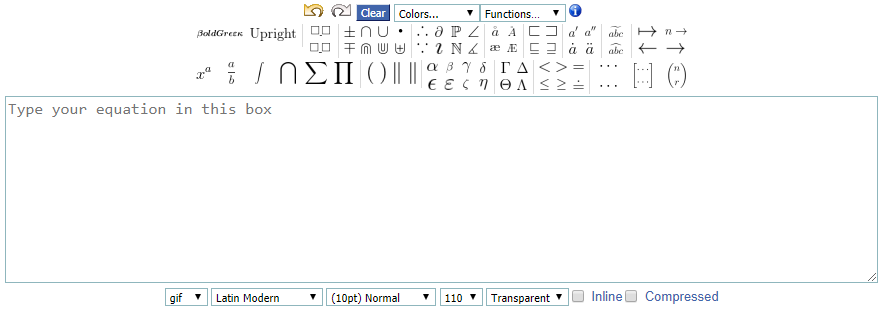
\includegraphics[width=.8\linewidth]{Images/equationeditor.png}
    \caption{Exemplo de editor de equação on-line}
    \label{fig:editor:eq}
\end{figure}

\subsection{Resumos}
Um artigo pode ter um resumo, e a classe \lstinline|article| provê um ambiente \lstinline|abstract|.
    

\section{Floats}
\subsection{O Que São Floats}

    \begin{outline}
        \1 Ambientes que o \LaTeX\ posiciona no melhor lugar possível de acordo com suas regras de diagramação.
        \2 figure
        \2 table
        \1 Permite opções que orientam o posicionamento do bloco formatado gerado pelo algoritmo
        \2 \textbackslash \{figure\}[hbt]
        \3 h -- here -- tenta colocar na posição onde o comando está em relação ao texto
        \3 b -- bottom -- tenta colocar no fim da página
        \3 t -- top -- tenta colocar no top da página
        \2 Essa é a melhor ordem, pois (quase) garante que a imagem não vai aparecer antes de ser citada
        \1 Flutuar significa que você não determina exatamente onde vão ficar, mas sugere ao algoritmo 
    \end{outline}


\subsection{O ambiente \lstinline|figure|}

Como o nome diz, o ambiente \lstinline|figure| serve para inserir figuras em seu texto. Como a maior parte das pessoas faz figuras fora do \LaTeX, mesmo havendo pacotes poderosíssimos de desenhos por comandos, ele é usado normalmente com o comando
\lstinline|\includegraphics[keyvals]{imagefile}|. Para isso é importante usar o pacote \lstinline|graphicx|, que possui ainda comandos para fazer operações na figura, como cortar e colocar em escala, como fazemos com a opção \lstinline|width| na \ref{fig:fig}.


\begin{figure}[hbt]
    \begin{LTXexample}[pos=b]
    \begin{figure}
    \centering
    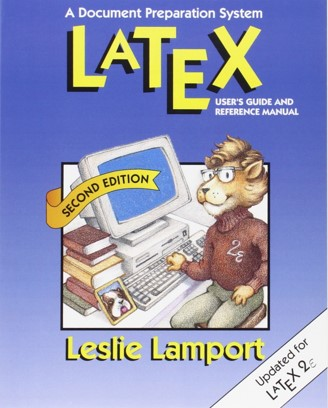
\includegraphics[height=0.3\textheight]{Images/Picture6}
    \caption{Capa do livro de \LaTeX\ }
    \label{fig:picture6}
\end{figure}
    \end{LTXexample}
    \caption{Exemplo de uso do ambiente figure.}
    \label{fig:fig}
\end{figure}

\subsection{Os ambientes \lstinline|tabular| e \lstinline|table|}

Para construir tabelas usamos o ambiente \lstinline|tabular|, porém, para permitir que o \LaTeX\ as coloque no lugar mais apropriado no texto, usamos o ambiente flutuante \lstinline|table|

\begin{figure}[hbt]
    \begin{LTXexample}[pos=b]
    \begin{table}
    \caption{Tabela de Idades}
    \centering
    \label{tab:idades}
    \begin{tabular}{|c|c|}
    \hline
    \textbf{idade} & \textbf{nome} \\
    \hline
    0-2   & bebê \\
    3-12  & criança \\
    12-19 & adolescente \\
    20-25 & jovem adulto \\
    25-60 & adulto \\
    60-80 & sênior \\
    80-   & terceira idade \\
    \hline
    \end{tabular}
    \end{table}
    \end{LTXexample}
    \caption{Exemplo de uso dos ambientes table e tabular.}
\label{fig:tabtab}
\end{figure}





